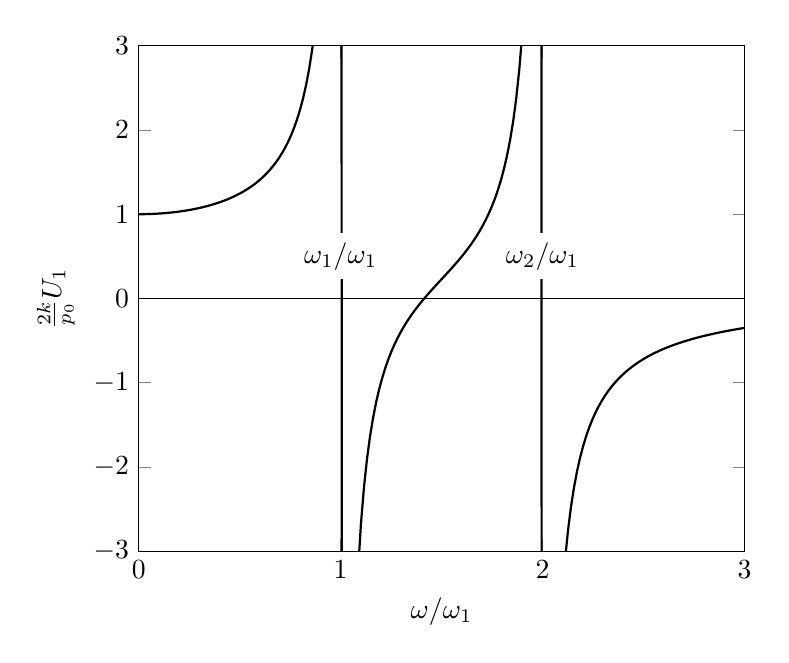
\begin{tikzpicture}
    \begin{axis} [
        height=8cm,
        ylabel = $\frac{2k}{p_0} U_1$,
        xlabel = $\omega/\omega_1$,
        xmin = 0, xmax = 3,
        ymin = -3, ymax = 3,
        xtick = {0, 1, 2, 3},
        ytick = {-3, -2, -1, 0, 1, 2, 3},
     ]
        \addplot [
            domain=0:3,
            samples=200,
            color=black,
            thick,
        ]{(1 - 0.5 * x^2)/((1-x^2) * (1-0.25 * x^2))};

        \node[rectangle,fill=white] at (1, 0.5) {$\omega_1/\omega_1$};
        \node[rectangle,fill=white] at (2, 0.5) {$\omega_2/\omega_1$};
        \draw[thin] (0, 0) -- (3, 0);
    \end{axis}
\end{tikzpicture}


